 
%
%  $Description: Author guidelines and sample document in LaTeX 2.09$ 
%
%  $Author: ienne $
%  $Date: 1995/09/15 15:20:59 $
%  $Revision: 1.4 $
%

\documentclass[times, 10pt,twocolumn]{scrartcl} 
\usepackage{ave}
\usepackage{times}
\usepackage{graphicx}
\usepackage{float}
\usepackage{url}

%\documentstyle[times,art10,twocolumn,latex8]{article}

%------------------------------------------------------------------------- 
% take the % away on next line to produce the final camera-ready version 
\pagestyle{empty}
\setkomafont{disposition}{\normalfont\bfseries}
%------------------------------------------------------------------------- 
\begin{document}

\title{JZX: Java 'Sinclair ZX Spectrum' emulator\\
Evaluation and Optimization of Emulation Engine\\
Group 7}

\author{Ant\'{o}nio Goul\~{a}o\\
66950\\
antonio.m.goulao@ist.utl.pt\\
%
\and
Jos\'{e} Correia\\
67026\\
jose.p.correia@ist.utl.pt
%
  \and
  Miguel Borges\\
  67041\\
  miguel.a.borges@ist.utl.pt\\
}

\maketitle
\thispagestyle{empty}

\begin{abstract}
  The ZX Spectrum was one of the most popular home computers in the United Kingdom and in Europe in the 80’s, as a consequence, many people now remember the days they played in a Spectrum while they were young. The ZX Spectrum is no longer produced, to break the nostalgia for this machine, many emulators appeared and among them is the JZX, a ZX Spectrum PC emulator written in Java. In this paper we present a study of the CPU and memory emulation, and we present several optimizations to it.\\
  \\
  \textbf{Keywords:} JZX, emulator, ZX Spectrum, virtualization.\\
\end{abstract}
%------------------------------------------------------------------------- 
\section{Introduction}
In this paper we propose to present a study of the ZX Spectrum home computer covering its system and memory architecture and study how this aspects of the original machine were emulated in the JZX emulator. Finally we propose to study the CPU emulation and apply several techniques to it, learned during the VEE course, in order to improve its performance.
%------------------------------------------------------------------------- 
\section{The ZX Spectrum}
The ZX Spectrum is an 8-bit generation personal computer released by Sinclair Research Ltd. It was first launched in the United Kingdom in 23rd April 1982 and discontinued in 1992. The ZX Spectrum was released as eight different models, from the 16KB RAM released in 1982 to the ZX Spectrum +3, released in 1987, with 128KB RAM and built in floppy disk drive. Like the Commodore 64, the ZX Spectrum was among the first mainstream audience home computers.

\subsection{System architecture}
The ZX Spectrum is based on a 3.54MHz Zilog Z80A CPU connected to a ULA responsible for all the interfaces (tape, sound, keyboard and video) and to an arrangement of three input/output buses. These buses are the Data Bus, the Address Bus and Control Bus. The CPU can address up to 64KB of memory. The first model came with a 16KB RAM followed by a 48KB RAM version and later by 128KB RAM versions. The ULA is able to bring the CPU to a temporary halt, giving it absolute priority and allowing it to access the standard RAM without interference from the CPU. The video output is through a RF modulator and has a 32x22 character text display with 256x192 pixel resolution and 8 colors. The sound in the 16/48KB models has one beeper capable of producing 1 channel with 5 octaves, the 128KB model was capable of producing 3 channels with 5 octaves.\\
\indent A T-state is the equivalent to the time length of one clock pulse to the CPU, in the case of the Z80, one T-state has the duration of 1/3500000 seconds. The T-states are used for synchronizing the rendering of screen lines that make one frame. In the 48K version there are 224 T-states/screen line (scanline) and 312 screen lines/frame. In the 128K version the number of T-states/screen line increases for 228 and the number of screen lines/frame decreases for 63.\\
\indent This CPU was an improvement to the 8080 with instruction set capable of performing bit manipulation, block move and block I/O, new index registers with instructions for direct base+offset addressing and a better interrupt system. Like on the 8080 the 8-bit registers are typically coupled to provide a 16-bit version.

\begin{figure}
	\center{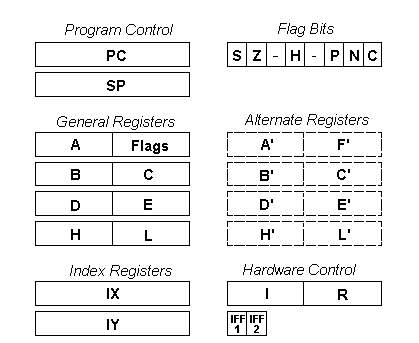
\includegraphics[width=0.4\textwidth]{img/z80_reg.png}}
	\caption{Z80 CPU registers.}
\end{figure}

\indent Z80 instructions are represent in memory as byte sequences with following forms:
\begin{itemize}
\item {[prefix byte,]  opcode  [,displacement byte]  [,immediate data]}
\item {two prefix bytes,  displacement byte,  opcode}
\end{itemize}
\indent The Z80 uses 252 codes as single byte opcodes (no prefix byte), the remaining four are used as opcodes prefixes: CBh and EDh enable extra instructions, DDh or FDh selects IX+displacement or IY+displacement. This are useful to access data organized in fixed structures but tend to be slower than using sequences of using HL register and increment it.\\
\indent The Z80 instructions are grouped into the following categories:
\begin{itemize}
\item {8-bit arithmetic and logic operations}
\item {16-bit arithmetic}
\item {8-bit load}
\item {16-bit load}
\item {Bit set, reset, and test}
\item {Call, return, and restart}
\item {Exchange, block transfer, and search}
\item {General purpose arithmetic and CPU control}
\item {Input and output}
\item {Jump}
\item {Rotate and shift}
\end{itemize}
\indent Z80 doesn’t have any multiply instruction available.

\subsection{Memory architecture}
The Z80 processor is a 8-bit CPU,but can operate 8-bit or 16-bit values, that allows index up to 64K of memory. The 48K Spectrum has 16K ROM and 48K RAM, meaning that the processor indexes directly  the memory. For the 128 and +2 Spectrums, there are two 16K pages of ROM and eight 16K pages of RAM. For the +3, +2A, +2B Spectrums there are twelve 16K pages, four pages for ROM and eight pages for RAM. From this ten and twelve pages, only four are visible to the CPU.\\
\indent The CPU addressable memory, from 0 (0000h) to 65535 (FFFFh) is slitted in four 16K areas. The lower 16K bytes of memory (0000h-3FFFh) are the ROM which holds the monitor program, divided between the input/output routines, the BASIC interpreter and expression handler. The next 16K bytes (4000h-7FFFh) are RAM used to hold the system variables, buffers and screen area. The last 32K (8000h-FFFFh) are RAM that provides extra memory space for the user.\\
\indent In the 128K versions, when the system boots, it maps the ROM 0 to the 0000h-3FFFh addresses, RAM 5 to 4000h-7FFFh addresses and RAM 2 and RAM 0 to 8000h-BFFFh and C000h-FFFFh addresses respectively. All the hidden memory becomes visible to the hardware using a method called paging.

\subsection{Paging}
We can send a combination of bits to an I/O port to select which memory page we want to use. The I/O address used to select the RAM page is at 32765 (7FFDh) address and accepts a 6-bit long number. Each bit in this number has its function, Bit 0 to Bit 2 selects which RAM page (0-7) goes to the highest seen addresses of the memory (C000h-FFFFh). Bit 3 switches screens. There is two RAM pages in memory that can hold a screen, RAM 5 (screen 0) and RAM 7 (screen 1). This operation does not change the content of RAM 5 which is always paged between 4000h and 7FFFh. Bit 4 selects which ROM is paged into lower addresses of the memory (0000h-3FFFh). For the Spectrum version with four ROM pages, this bit is used in combination with bit 2 of port 1FFDh. In the versions of Spectrum with two ROMs, ROM 0 contains the 128K editor and menu, ROM 1 contains the 48K BASIC. For the versions with four ROMs, ROM 0 contains the 128K editor, ROM 1 contains the 128K syntax checker, ROM 2 contains +3DOS and ROM 3 contains the 48K BASC. Bit 5 function is to disable paging operations, if this bit is set, paging operations will no longer work and the machine will assume the 48K configuration. To turn the machine back to the 128K configuration, this must be switched off or reseted.\\
\indent From the +3 and followings, the I/O port 1FFDh is used for ROM and RAM switching with a 5-bit long number. Bits 0 and 1 are used for ROM/RAM switching, the value in bit 2 affects how bits 0 and 1 work in RAM/ROM switching operations. Bit 3 is related with the disk motor and bit 4 with the printer strobe.\\
\indent When bit 0 is 0 in port 1FFDh, combining bit 4 in port 7FFDh and bit 2 in port 1FFDh we can form a 2-bit number, bit 4 is the least significant bit and bit 2 the most significant bit, which decides which ROM is paged to lowest memory addresses (0000h-3FFFh).
\begin{table}[h]
\centering
	\begin{tabular}{|{c}|{c}|{c}|}
	\hline
	& Bit 2 1FFDh & Bit 4 7FFDh \\ \hline
	ROM 0 & 0 & 0 \\ \hline
	ROM 1 & 0 & 1 \\ \hline
	ROM 2 & 1 & 0 \\ \hline
	ROM 3 & 1 & 1 \\ \hline
\end{tabular}
\caption{ROM switching}
\end{table}

\indent When bit 0 in port 1FFDh has the value 1, bits 1 and 2 are used to perform a special paging mode in which all four pages in memory contain RAM. These are the possible combinations:
\begin{table}[h]
\centering
\begin{tabular}{|{c}|{c}|{c}|}
	\hline
	& Bit 2 1FFDh & Bit 1 1FFDh \\ \hline
	Mode 0 & 0 & 0 \\ \hline
	Mode 1 & 0 & 1 \\ \hline
	Mode 2 & 1 & 0 \\ \hline
	Mode 3 & 1 & 1 \\ \hline
\end{tabular}
\caption{Bit combination}
\end{table}
\begin{table}[h]
\centering
\begin{tabular}{|p{1,2cm}|{c}|{c}|{c}|{c}|}
 \hline
	& Mode 0 & Mode 1 & Mode 2 & Mode 3 \\ \hline
	0xFFFFh - 0xC000h & RAM 3 & RAM 7 & RAM 3 & RAM 3 \\ \hline
	0xBFFFh - 0x8000h & RAM 2 & RAM 6 & RAM 6 & RAM 6 \\ \hline
	0x7FFFh - 0x4000h & RAM 1 & RAM 5 & RAM 5 & RAM 7 \\ \hline
	0x3FFFh - 0x0000h & RAM 3 & RAM 4 & RAM 4 & RAM 4 \\ \hline
\end{tabular}
\caption{Extended memory paging}
\end{table}
%\section{The ZX Spectrum}
%\begin{itemize}
%\item\textbf{Name:} JZX\\
%\item\textbf{URL:} \url{http://www.sonic.net/~surdules/projects/jzx/}\\
%\item\textbf{VM Type:} System-VM\\
%\item\textbf{Common Usage:} A common ZX Spectrum emulator that can be used in any platform that runs Java. This Virtual Machine is capable of emulating the machine's interpreter and run the existent programs in its time.\\
%\item\textbf{Motivation:} This project will allow us to acquire a deeper knowledge of how a System-VM works inside. This project was last updated in 2006 and has a basic emulation process that we pretend to improve and provide a tool to analyze which operations are more used.\\
%\end{itemize}

%------------------------------------------------------------------------- 
\section{The JZX Emulator}
The JZX Emulator is the ZX Spectrum emulator implemented in Java. This is the studied emulator and the one we performed some optimizations described below.
Razvan Surdulescu is a Staff software engineer ate Google, graduated from Harvard University and University of Texas at Austin who took the challenge of building a ZX Spectrum emulator written 100\% in Java. This emulator is based on a Linux native emulator called XZX.
To emulate the ZX Spectrum, each hardware component must be a logical component made in Java, to correctly simulate the execution. Thus, in our emulator, each Spectrum component is a class that inherits from the abstract class BaseComponent. It is used a composite pattern, where the component BaseSpectrum is the composite, and the other components are the leafs, that allows BaseSpectrum to be the abstraction for all components. The Spectrum components are: BaseSpectrum, BaseMemory, Z80, BaseIO, BaseKeyboard and  BaseScreen.
The emulator emulates two different versions of the ZX Spectrum, the 48K model and the 128K. Since the machines are similar, the author made 95\% of the code base shared by the two versions.
It does emulate the normal behavior of the ZX Spectrum including the sound and the ROM reading but doesn't emulate the tape reader, because the original uses it to load the and save the software and the emulator uses .z80 files, nor the speaker.
\begin{figure}
	\center{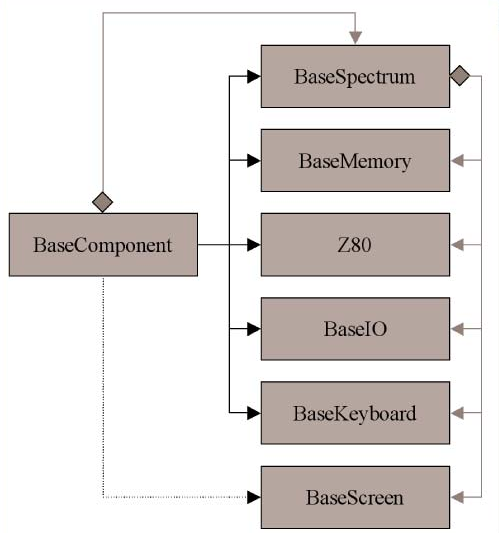
\includegraphics[width=0.4\textwidth]{img/softwareArchitecture.png}}
	\caption{Software architecture.}
\end{figure}

\subsection{CPU Emulation}
The ZX Spectrum emulator is very simple and is based on a decode-and-dispatch interpreter. It maintains the general registers, the program counter, stack pointer and flag registers in memory having an integer variable for each register.
The emulator has a interpretation loop that follows the execution of the program by fetching the memory position pointed by the program counter and then comparing the opcode with all the possible opcodes of the processor in order to discover which instruction should be executed. That comparison is done in a switch case that is not even ordered by the most used instructions. 
All the code for each instruction is placed inside the respective case statement. This very basic parsing is a major source of inefficiency since for each original instruction the emulator need to perform N comparisons and only then it emulates the instruction. 
Like in the original processor, each time an instruction is executed all the flags are updated. This causes a lot of inefficiency since most of the times the work performed to update the flags is bigger than the work to execute the instruction itself.
After fetching and executing an instruction the emulator updates the screen and makes a sleep so that the compatibility with the original processor programs are maintained. The time of the sleep depends on the instruction that has been executed. As we optimize the emulation process of the instructions we expect that the update step occupies more time because the total time for each instruction need to be maintained.
As you can see the original emulator has lots of inefficiencies and some of them could be reduced by applying techniques learned in the AVE course. In the next section we present some of the possible optimizations.

\subsection{128KB Memory Emulation}
The emulator uses two arrays to emulate the memory of the physical machine. The m\_frame array is the memory visible to the CPU, with only four positions, and the m\_page array its all the available memory that the 128K versions had, with twelve positions. Each position in those arrays has 16KB like the physical pages in the originals had.
The first position of the m\_frame its where the ROM pages are loaded. The remaining pages are RAM pages with the same distribution of the original. In the m\_page array, the first four positions are ROM pages and the remaining are RAM pages. This pages are filled with data during the load of the .z80 file.

Paging
Like the 128K ZX Spectrum versions do, this emulator is able to do paging too.
The following code takes advantage of a known bug in the original 128K ZX Spectrum. This code activates the second screen, stored in memory at address 7C00h, and writes small files to the RAMdisk causing it to fail in recognizing the existence of the second screen. Type the following code in the 128 BASIC:\\
10 POKE 23388, 24: REM\\
20 FOR I = 1 TO 562\\
30 SAVE! ''F'' + STR\$ I CODE 0, 1\\
40 NEXT I\\
50 PAUSE 0\\
60 POKE 23388, 16: REM\\
RUN\\
As you may noticed, this code begin to fill the screen with colorful squares form bottom to top. If you now type POKE 23388,24: PAUSE 1000 and press enter you will see the screen that the previous chunk of code fill with colorful squares. During the execution of the previous chunk of code the emulator is constantly paging the memory.

%\section{Internal Mechanisms Study}
%  The main focus of our work in this System-VM is to study the mechanism of code emulation so we can improve it, and study the memory emulation mechanism.

%------------------------------------------------------------------------- 
\section{Optimization Techniques}
In this section, we briefly analyze some possible improvements to the CPU emulation of the emulator, then we will show which of the optimizations we made and optimizations that we tried to implement but didn't work.

\subsection{Pre-decoding}
Every time the emulator prepares to execute the next instruction, it needs to perform multiple accesses to the memory in order to get all the necessary values to execution of the instruction. For instance, when trying to load a value to a register, the emulator needs to get the opcode of the instruction pointed by the program counter, then read the value of the register and last, read the value. This could be avoided if every time the emulator is reading from a new memory position that was never executed before, it saved the unchanged values, like the opcode and the register number into a cache. The next time this instruction would be performed, less memory accesses would be needed, improving the emulator's performance.
We tried this approach, but due to the paging mechanism of the emulator, the cache needed to be cleaned every time a page changed occurred.

\subsection{Indirect Threading}
For each execution of the decode loop, the emulator uses an enormous switch/case statement to match and execute and instruction. this bad in terms of code location because we are constantly jumping between distinct code zones. It could be avoided if in the end of each instruction, the emulator seek on a table which would be the next instruction to be executed, jump to it and execute it.

\subsection{Switch/case removal}
As we said, each time an instruction is to be decoded the emulator performs a comparison of the instruction opcode with all the possible opcodes until it finds a match. We can remove this overhead by having a table of instructions ordered by the opcode. Each time the emulator needs to discover which operation to execute it only needs to access one position of the table and execute the instruction.

\subsection{Lazy flags}
Each time an instruction is executed it updates the values of the affected flags. The work of updating the flags is sometimes bigger than executing the instruction itself and most of the times the flags values are not used. We can remove this source of overhead by calculating the flags in a lazy way. That is, none of the instructions updates the flags and when an instruction need to use a flag value, it calculates the value for that flag.

\subsection{Parallel update and emulate}
In the decode and dispatch loop each time an instruction is executed the emulator updates the screen and makes a sleep to maintain compatibility with the original processor but when it returns from the sleep it need to wait for the instruction to be executed. This work could be made in parallel, that is, we could execute the instruction at the same time we are waiting for the next screen update and with this, when the sleep ends we already have the next instruction executed and we could update and sleep again. With this approach we would have zero time for executing the instructions because that time would be overlapped by the time of sleep and updates.

\subsection{CPU Emulation}
Here, we present all the improvements performed to the emulator. All but one, the last, were implemented successfully, the reasons for that will be addressed later.

\subsubsection{Instructions array}
In the original implementation, each time an instruction is to be decoded it compares the opcode of that instruction with all the possible opcodes. This was done in an enormous switch case that was not even sorted by the most used instructions and so in the worst case the emulator needed to do N comparisons for each original instruction (being N the total number of instructions of the Z80). All the code that implements an instruction was on the respective case statement. This could be good because it has no indirection level for the execution of the instruction code but the number of comparisons and branches that needs to be performed in the switch statement totally overlaps this. 
As you can intuitively say, this was a major source of inefficiency and so we needed to change the way of decoding an instruction.
We choose to have an array of instructions in witch the position of a given instruction is the same as the opcode for that instruction. this is possible because we only have 255 main instructions. There are some instructions like the EDh FDh and DDh that use a bigger opcode and so we use an extra level of indirection maintaining the switch statement for this kind of instructions. This is not problematic because this instructions are originally the less used.
For each of the main instructions we created a new instruction class with the original code that was on the switch statement and so the behavior was not affected. Each of the positions of the instructions array is an instruction instance that knows how to emulate the original instruction.
In this way we can totally remove the original switch statement that needed to perform in the worst case O(N) comparisons by an access to a position in the array O(1).



\subsubsection{Lazy flags}
The original processor updates the flags on each instruction execution. This has no extra cost for the processor because this flags are updated has the result of the instruction execution. The original emulator implementation, directly emulates this behavior by updating the respective flags on each instruction execution. Each flag update is done by calling a CPU operation that was implemented in a method for each operation.
The original implementation has an big cost because most of the times the number of real instructions needed to update the flags is bigger than the ones needed to execute the instruction and the flag values are very rarely used by the next instructions. So, most of the work performed was in vague.
We improved this part of the emulator by calculating the flags in a lazy way, that is, the emulator never calculates the flag values until they are used. This can be done by saving the last operation that updates each flag and saving the values needed to calculate his value.
As each operation that updates the flags was performed in a method we needed to refactor this and each of them is now implemented in a operation class that has a method for getting the value of each flag and is then used like the original one. Each operation knows how to get the values needed to calculate the flags, knows how to calculate them and witch of the flags it should update.
Instead of having a field for each flag we have an array of operations, in a way that each flag is represented by a position in the array and each position of the array has the last operation that updates that flag. When an operation is executed, the operation is saved in the right array position and when the emulator needs to know the value of a flag it accesses the respective position on the array and calculates the value for that flag.

\subsubsection{Parallel emulate}
The decode loop of the emulator does the emulation of a given instruction and after that it performs updates to the screen and waits a time that depends on the executed instruction (fig X). By profiling the code we concluded that the emulator spent about 30\% emulating the instruction and 70\% updating and waiting.
In theory, if we parallelize the two tasks, we could eliminate 30\% of the total time because the time of emulating would be overlapped by the time of updating (fig Y). This can be done because while the update task is waiting the emulator is actually doing nothing and there are no dependencies between the two tasks.
We modified the original loop so that while one thread is updating the screen and waiting as result of executing a given instruction N the other task is emulating the next instruction N+1. This way we expect to gain some time if we have a machine with at least two cores.
The two tasks need to be synchronized, that is, we can't emulate more than one instruction for each update nor we can update more than one time for each instruction. This synchronization part is important because if the synchronization takes too much time, we end up gaining nothing by having two threads. We tried to implement several mechanisms of synchronization and we discovered that we can't put one of the threads to sleep while waiting for the other. If we do that, we end up by having an emulation process that is so slow that the emulator stops working normally. The solution was to have active wait to synchronize the two threads using a volatile variable. In this solution we are spending CPU time to then gain some time on the emulation process, that should be almost zero time, that is, we are exchanging available computation power in exchange for performance.

\subsubsection{Code cache}
Each time an instruction is executed the emulator is pessimistic and do all the process of decoding and executing that instruction. This includes the costly operations of reading from memory. We tried to improve this by having an instructions cache where the memory values needed to execute a given instruction where saved and then reused when the instruction was executed again. In this way we would only read from memory the needed values one time and we expected that this improves the execution of the emulator. We had some implementation issues related with the paging mechanism that does not allow us to directly associate the PC with the instruction because the original page can be switched out by another page of code. We had no time to solve this issues and so we removed the caching mechanism however we can suggest a way to turn solve this issue.
We can solve this issue by associating the values in cache not only with the memory position but also with the number of actual the page in memory. This way we would never have to clean the cache when changing between memory pages.
%\section{Project Approaches}
%In the first place we will need to analyze the actual implementation of the emulator and understand its mechanisms of emulation. In particular we will study the memory mapping mechanisms used in the actual implementation. This first part has as objective discover ways in which we can optimize the actual implementation of the emulator.
%
%After that we will apply techniques learned in the course in a way that improve the emulator. The main focus will be in optimizing the code decoding of the actual solution. To do that, we pretend to implement basic predecoding. 
%The actual emulation procedure uses a switch statement, it is inefficient because the same instruction is analyzed every time it is executed. Our main focus is to analyze an instruction once and save it for later uses, simplifying interpretation and speeding it up. This procedure will raise memory consumption, but still acceptable according to the memory available in computers nowadays.
%While studying the code we will also study the documentation provided by the main developer of the emulator to helps us find places where we can improve it.
%
\section{Evaluation}
To evaluate the improvements and optimizations made to the JZX, we tested three versions, the original implementation, the array instruction implementation and the lazy flags implementation, to measure the time spent during the execution of an instruction. All the three implementation tested are single thread versions. To evaluate the emulator with multiple threads, we tested two versions, single thread version, and two threads version. Both versions with lazy flags. The tests consisted in playing two ZX Spectrum games,  Bombjack, 48K game, and Renegade, 128K game, for about five minutes. This tests were made in RNL's computer, with Intel Core i5 760 (Quad-core) CPU, and 8 GB of memory, running Debian 6.0 and Oracle's Java 6 JVM.

\subsection{Instruction execution}
To measure the time that each instructions takes to execute, we use the average time that two million instructions take to execute. We measure the time that every instruction takes to execute in nanoseconds and after two million instructions executed we compute the average that every instruction took to execute. With this approach we can execute and compare the performance between versions without affecting the performance of the emulator.\\
\indent In Figure 5, we present the chart that shows the evolution of the time per instruction in the Bombjack, 48K game. The value of time in original implementation, is much higher than the other versions. The time per instruction in instruction array version improved about 47\% compared to original version. Regarding the lazy flags version, we were hoping that the time per instruction had decreased, but the value of time had a slight increase of about 3\%.\\
\indent Like in Bombjack, in Renegade, a 128K game, in the original version the value of time per instruction is also higher than the improved versions. In this game, the improvement is about 43\% compared to the array instruction version. As in Bombjack, the version with lazy flags should be more efficient, but the value of time increased about 7\%.\\
\indent The lazy flags implementation goal was to make the execution of one instruction faster. But in practice, it didn't happened. This is due to a choice in our implementation. The problem lies in when we execute one instruction, instead of directly access the position in the flags array, we perform a for cycle to do that.\\
\indent As we said earlier, the goal of the implementation with threads was eliminate 30\% of the total time.\\
\indent The charts in figures x and y show that the improvement of having two threads, one processing the execution of one instruction and the other processing the update of the screen, doesn't have great impact in the total emulation time. Due to active waits the emulation time still occupies some time between execution time, making the emulation sequential.
\begin{figure}
	\center{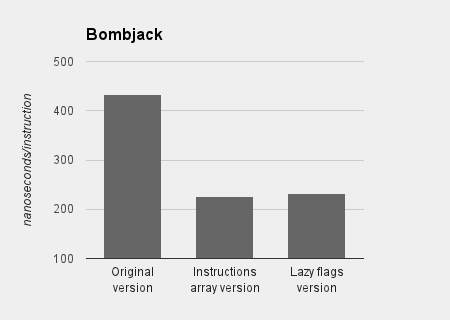
\includegraphics[width=0.4\textwidth]{img/chart_1.png}}
	\caption{Time per instruction in Bombjack}
\end{figure}
\begin{figure}
	\center{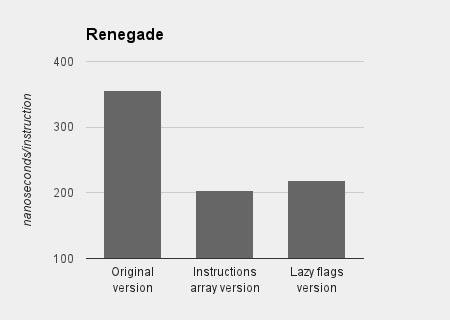
\includegraphics[width=0.4\textwidth]{img/chart_2.png}}
	\caption{Time per instruction in Renegade}
\end{figure}
\begin{figure}
	\center{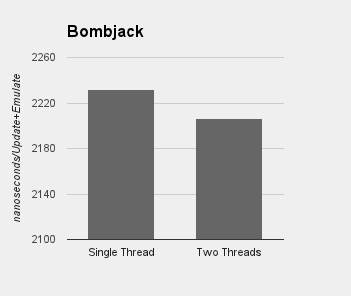
\includegraphics[width=0.4\textwidth]{img/chart_3.png}}
	\caption{Comparison time per instruction in Bombjack}
\end{figure}
\begin{figure}
	\center{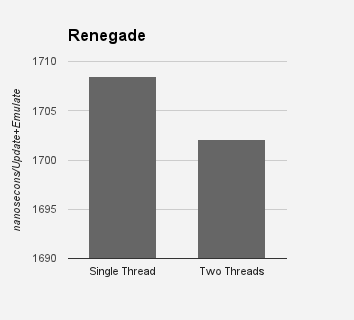
\includegraphics[width=0.4\textwidth]{img/chart_4.png}}
	\caption{Comparison time per instruction in Renegade}
\end{figure}
%\section{Evaluation}
%Along the way of the project we will apply benchmark techniques so that we can the best solutions. We will test the number of bytecodes executed and the number of frames per second before and after implement our solution. The tests will be performed using 128KB games.
%
%\section{Detail Section}
%This emulator is written in Java, so the project will be executed using this language.
%The changes proposed here, will use the algorithms and techniques presented in the lectures and in the course's bibliography.
%
\section{Future Work}
Our work made some progresses to this emulator but we left some work to be done yet. Get a solution to remove the active waits in the emulator, thread operations like wait or sleep lower the performance of the emulator, but with a working multithread solution the emulation time is 100\% update time. Change the necessary variables to short or implement a short array in order to save memory. For the pre-decoding id could be tried to store the memory position plus its page or limit it to the 48K version of the emulator.
%------------------------------------------------------------------------- 
\section{Conclusion}
In the end, after many hours trying to understand the emulator, after improvements and setbacks, we achieved our main goals, apply what we have learned in the VEE course to a real emulator and decrease the execution time of each instruction. In return we increased the CPU use by the emulator, but we believe that with more time we could revert this increase. We believe too that the cache implemented only in the 48K version of the emulator would perform some earnings, instead of the version we implemented applied to both versions of the emulator.
The overall is we managed to apply or we tried to apply real improvements to a real emulator, still, not all of them remained in the final version.
%\section{Conclusion}
%At the checkpoint, we expect to have a good overview of how the emulator is implemented and have a strategy ready to implement. After concluding this project we hope to have a better understanding of the virtualization mechanisms used in the emulator. We hope to improve the performance and give an important contribute to this project.

\bibliographystyle{ave}
\bibliography{ave}

\begin{thebibliography}{1}

  \bibitem{notes} R. Surdulescu. {\em JZX: Java 'Sinclair ZX Spectrum' emulator}  \url{http://www.sonic.net/~surdules/projects/jzx/}.
  \bibitem{notes} C. Lawson, Amstrad. {\em The Sinclair ZX Spectrum +3}  \url{http://www.worldofspectrum.org/ZXSpectrum128+3Manual/}.
  \bibitem{notes}{\em Bugs in the rom}  \url{http://nonowt.com/magfold/articfol/bugs_in.html}.

\end{thebibliography}

\end{document}

